\documentclass[aspectratio=169,11pt]{beamer}

\usepackage[T1]{fontenc}
\usepackage{lmodern}
\usepackage{amsmath,amssymb}
\usepackage{graphicx}
\usepackage{booktabs}

% figures live at the repo root
\graphicspath{{figs/}{../../}}

% ---------------------------------------------------------------- look
\definecolor{ink}{HTML}{1A1A19}
\definecolor{soft}{HTML}{52514E}
\definecolor{mblue}{HTML}{2A78D6}
\definecolor{morange}{HTML}{EB6834}
\definecolor{mgreen}{HTML}{199E70}
\definecolor{tint}{HTML}{F4F4F1}

\usetheme{default}
\usefonttheme{professionalfonts}
\setbeamertemplate{navigation symbols}{}
\setbeamercolor{normal text}{fg=ink,bg=white}
\setbeamercolor{structure}{fg=mblue}
\setbeamercolor{frametitle}{fg=ink}
\setbeamercolor{title}{fg=ink}
\setbeamercolor{subtitle}{fg=soft}
\setbeamercolor{author}{fg=soft}
\setbeamercolor{date}{fg=soft}
\setbeamercolor{footline}{fg=soft}
\setbeamercolor{block title}{fg=white,bg=mblue}
\setbeamercolor{block body}{fg=ink,bg=tint}
\setbeamerfont{frametitle}{series=\bfseries,size=\large}
\setbeamerfont{title}{series=\bfseries,size=\LARGE}
\setbeamertemplate{itemize items}[circle]
\setbeamertemplate{frametitle}{\vspace{0.6em}\insertframetitle\par\vspace{-0.35em}{\color{mblue}\rule{2.2cm}{1.2pt}}}
\setbeamertemplate{footline}{\hfill\usebeamercolor[fg]{footline}\scriptsize\insertframenumber\hspace{1.2em}\vspace{0.8em}}
\setlength{\leftmargini}{1.2em}

\newcommand{\hl}[1]{{\color{mblue}\textbf{#1}}}
\newcommand{\ho}[1]{{\color{morange}\textbf{#1}}}
\newcommand{\src}[1]{}
\newcommand{\fullfig}[2][0.98]{\begin{center}\includegraphics[width=#1\textwidth,height=0.64\textheight,keepaspectratio]{#2}\end{center}\vspace{-0.6em}}

\title{Unexpected and expected shocks\\[0.2em]under time to produce}
\date{October 2026}

\begin{document}

\begin{frame}[plain]
  \vspace{2.2em}
  \titlepage
\end{frame}

% ==================================================================== MODEL
\begin{frame}{Household}
  \[
    \max\;\sum_{t}\beta^t\,\Xi_t\Bigl[\frac{C_t^{1-\gamma}}{1-\gamma}
      -\chi\frac{L_t^{1+\eta}}{1+\eta}\Bigr]
    \quad\text{s.t.}\quad
    P_tC_t+B_t=W_tL_t+(1+i_{t-1})B_{t-1}+\Pi_t
  \]
  \[
    \Xi_t\frac{C_t^{-\gamma}}{P_t}=\beta(1+i_t)\,\Xi_{t+1}\frac{C_{t+1}^{-\gamma}}{P_{t+1}},
    \qquad\qquad
    \frac{W_t}{P_t}=\chi L_t^{\eta}C_t^{\gamma}
  \]
  \medskip
  $\Xi_t$: demand shock.\quad $\gamma=2,\ \eta=2,\ \chi=1,\ \rho=1\%$.
\end{frame}

% --------------------------------------------------------------------
\begin{frame}{Final good}
  \[
    Y_t=\Bigl(\sum_i y_{i,t}^{\frac{\sigma-1}{\sigma}}\Bigr)^{\frac{\sigma}{\sigma-1}},
    \qquad
    y_{i,t}=\Bigl(\frac{p_{i,t}}{P_t}\Bigr)^{-\sigma}Y_t,
    \qquad
    P_t=\Bigl(\sum_i p_{i,t}^{1-\sigma}\Bigr)^{\frac{1}{1-\sigma}}
  \]
  \medskip
  Competitive.\quad $\sigma=5$.
\end{frame}

% --------------------------------------------------------------------
\begin{frame}{Intermediate producers}
  Labour hired at $t$ delivers $\Delta$ periods later:
  \[
    y_{i,t}(\Delta)=\kappa^{\Delta}\,(\Delta+N_i)\,A_t\,l_{i,t}
  \]
  Competitive, price-taking:
  \[
    \max_{\Delta,\;l_{i,t}}\;
    p_{i,t+\Delta}\Bigl(\prod_{j=t}^{t+\Delta-1}\frac{1}{1+i_j}\Bigr)\,y_{i,t}(\Delta)-W_t\,l_{i,t}
  \]
  $A_t$: TFP shock, dated at hiring.
\end{frame}

% --------------------------------------------------------------------
\begin{frame}{Delay and price}
  \begin{columns}[T,onlytextwidth]
    \begin{column}{0.46\textwidth}
      \textbf{Delay}
      \[
        \tau_i=\arg\max_{\Delta}\;(\beta\kappa)^{\Delta}(\Delta+N_i)
      \]
      \[
        \Delta_i^{*}=-\frac{1}{\log(\beta\kappa)}-N_i
      \]
    \end{column}
    \begin{column}{0.5\textwidth}
      \textbf{Price} (zero profit)
      \[
        p_{i,t}=\frac{W_{t-\tau_i}\prod_{j=t-\tau_i}^{t-1}(1+i_j)}{\zeta_i\,A_{t-\tau_i}}
      \]
      \[
        \zeta_i=\kappa^{\tau_i}(\tau_i+N_i)
      \]
    \end{column}
  \end{columns}
  \bigskip
  Rate enters unit cost: \hl{cost channel}.
\end{frame}

% --------------------------------------------------------------------
\begin{frame}{Ideal price index}
  Fixed wage, $W_t=W$:
  \[
    P_t=\Bigl(\sum_i p_{i,t}^{\,1-\sigma}\Bigr)^{\frac{1}{1-\sigma}}=\frac{W}{\tilde A_t},
    \qquad
    \tilde A_t=\Biggl(\sum_i\Bigl[\zeta_i\,A_{t-\tau_i}\prod_{j=t-\tau_i}^{t-1}\frac{1}{1+i_j}\Bigr]^{\sigma-1}\Biggr)^{\frac{1}{\sigma-1}}
  \]
  \medskip
  Steady state, $i=\rho$:
  \[
    \tilde A=\Bigl(\sum_i\bigl(\beta^{\tau_i}\zeta_i\bigr)^{\sigma-1}\Bigr)^{\frac{1}{\sigma-1}}
  \]
  \medskip
  $P_t$ moves only with rates and TFP over the last $\max\tau_i$ periods:\quad \hl{$\pi_t=-\Delta\log\tilde A_t$}.
\end{frame}

% --------------------------------------------------------------------
\begin{frame}{Market clearing}
  \[
    C_t=Y_t,\qquad\qquad
    L_t=\sum_i l_{i,t}=\sum_i\frac{y_{i,t+\tau_i}}{\zeta_iA_t},\qquad\qquad B_t=0
  \]
  \medskip
  Employment at $t$ produces deliveries at $t+\tau_i$.
\end{frame}

% --------------------------------------------------------------------
\begin{frame}{Labour today, output today}
  \[
    \text{\hl{Output at $t$}}:\quad
    Y_t=\Bigl(\sum_i\bigl(\zeta_i\,A_{t-\tau_i}\,l_{i,t-\tau_i}\bigr)^{\frac{\sigma-1}{\sigma}}\Bigr)^{\frac{\sigma}{\sigma-1}}
    \qquad\text{labour hired at } t-\tau_i
  \]
  \[
    \text{\ho{Labour at $t$}}:\quad
    L_t=\sum_i l_{i,t},\qquad
    \zeta_i\,A_t\,l_{i,t}=y_{i,t+\tau_i}
    \qquad\text{delivered at } t+\tau_i
  \]
\end{frame}

% --------------------------------------------------------------------
\begin{frame}{Time to build in the data}
  \begin{columns}[c,onlytextwidth]
    \begin{column}{0.66\textwidth}
      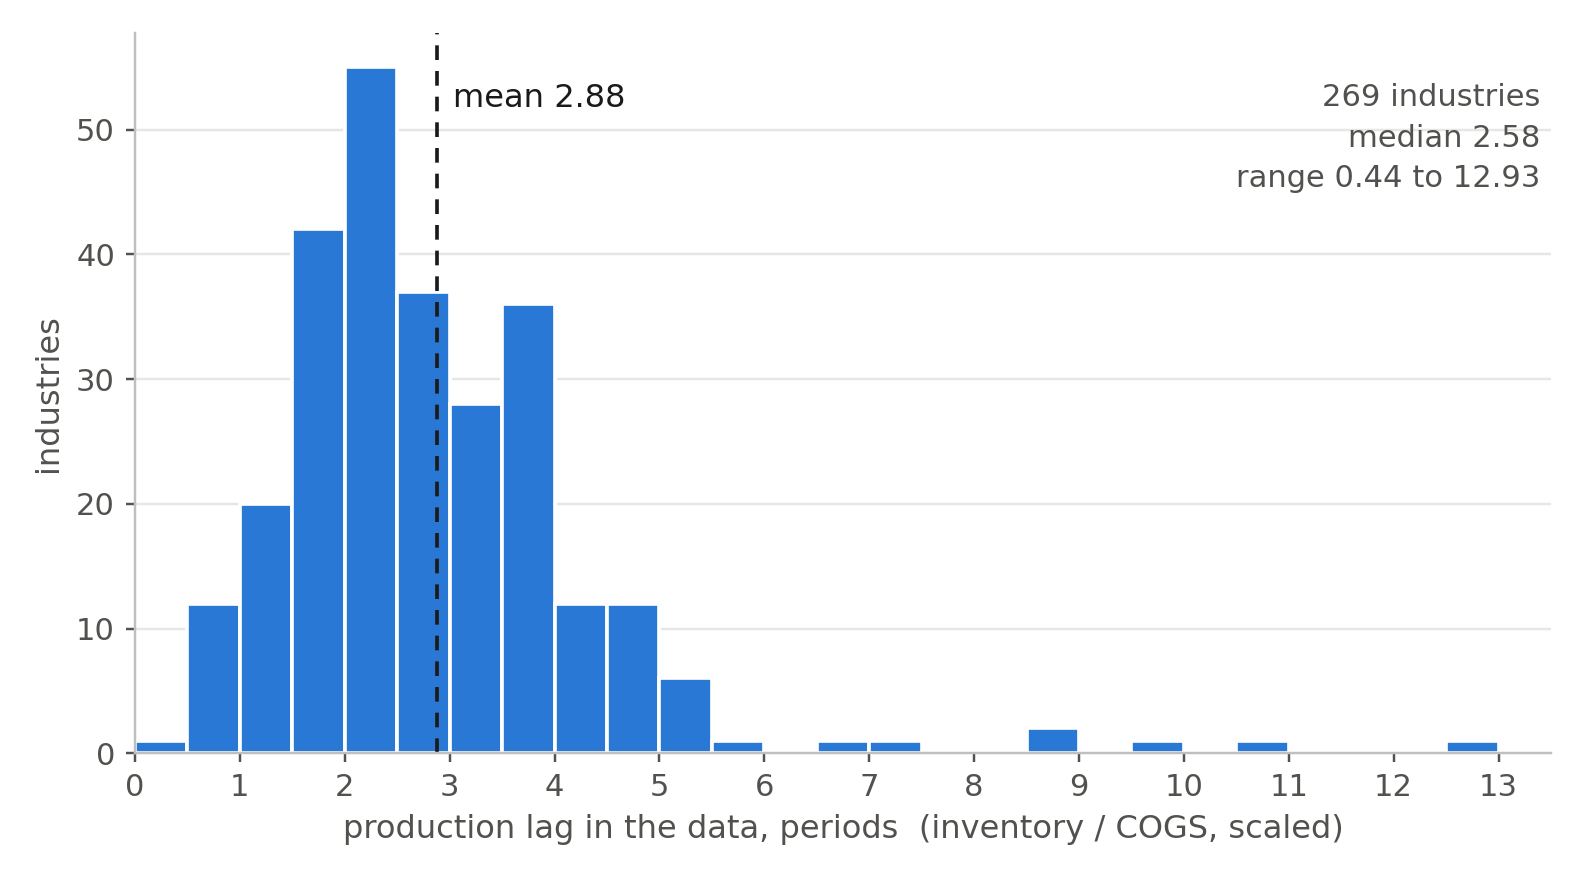
\includegraphics[width=\textwidth]{lag_distribution_data.png}
    \end{column}
    \begin{column}{0.3\textwidth}
      \begin{itemize}\setlength{\itemsep}{0.7em}
        \item Inventory/COGS, 269 industries
        \item $N_i$ matches each lag
        \item $\kappa=0.9018$
        \item Model: $\tau_i\in\{0,\dots,13\}$, mode 2
      \end{itemize}
    \end{column}
  \end{columns}
\end{frame}

% ==================================================================== PART I
\begin{frame}[plain]
  \vfill
  {\usebeamerfont{title}\color{ink}Expected shocks\par}
  \smallskip
  {\Large\color{mblue}Optimal rate path\par}
  \vfill
\end{frame}

% --------------------------------------------------------------------
\begin{frame}{Planner's problem}
  \[
    \max_{\{i_t\}}\;U=\sum_t\beta^t\,\Xi_t\bigl[u(C_t)-\chi\,v(N_t)\bigr]
  \]
  \[
    c^e_t=\varphi_{ya}\,a_t,\qquad \varphi_{ya}=\frac{1+\eta}{\gamma+\eta}=0.75,
    \qquad
    r^n_t=\rho+\gamma\,\Delta y^n_t-\text{dem}_t,\qquad \pi_t=-\Delta\tilde a_t
  \]
  \medskip
  \begin{itemize}
    \item Shocks: TFP $-3\%$, demand $-1\%$
    \item No welfare cost of inflation
  \end{itemize}
\end{frame}

% --------------------------------------------------------------------
\begin{frame}{Channel: a rate cut lowers prices for $\max\tau_i$ periods}
  $i_0=0.5\%$ for one period, no shock.

  \medskip
  \centering
  \begin{tabular}{lrrrrrr}
    \toprule
    $t$ & 0 & 1 & 2 & 3 & 4 & 5\\
    \midrule
    $\log P_t$, \% & $-0.495$ & $-0.437$ & $-0.258$ & $-0.134$ & $-0.045$ & $-0.012$\\
    $\pi_t$, \% & $-0.495$ & $0.058$ & $0.179$ & $0.124$ & $0.089$ & $0.033$\\
    \bottomrule
  \end{tabular}

  \bigskip
  \raggedright
  Prices move for \hl{13 periods}. A cut is deflationary.
\end{frame}

% --------------------------------------------------------------------
\begin{frame}{Expected TFP shock (3\%)}
  \fullfig{semi_endo_new_fixed_planner_A.png}
  \begin{itemize}
    \item Peg too loose: $c$ trough $-0.53\%$, efficient $-0.81\%$
    \item $i=0.83,\ 1.00,\ \hl{1.30},\ 1.04,\ 1.06\,\%$
  \end{itemize}
\end{frame}

% --------------------------------------------------------------------
\begin{frame}{Expected demand shock (1\%)}
  \fullfig{semi_endo_new_fixed_planner_demand.png}
  \begin{itemize}
    \item $i=\ho{0.34},\ \ho{1.27},\ 1.06,\ 1.00\,\%$: cut, then overshoot
    \item Hike undoes the deflation from the cut
  \end{itemize}
\end{frame}

% --------------------------------------------------------------------
\begin{frame}{Time to build vs none}
  \begin{columns}[c,onlytextwidth]
    \begin{column}{0.72\textwidth}
      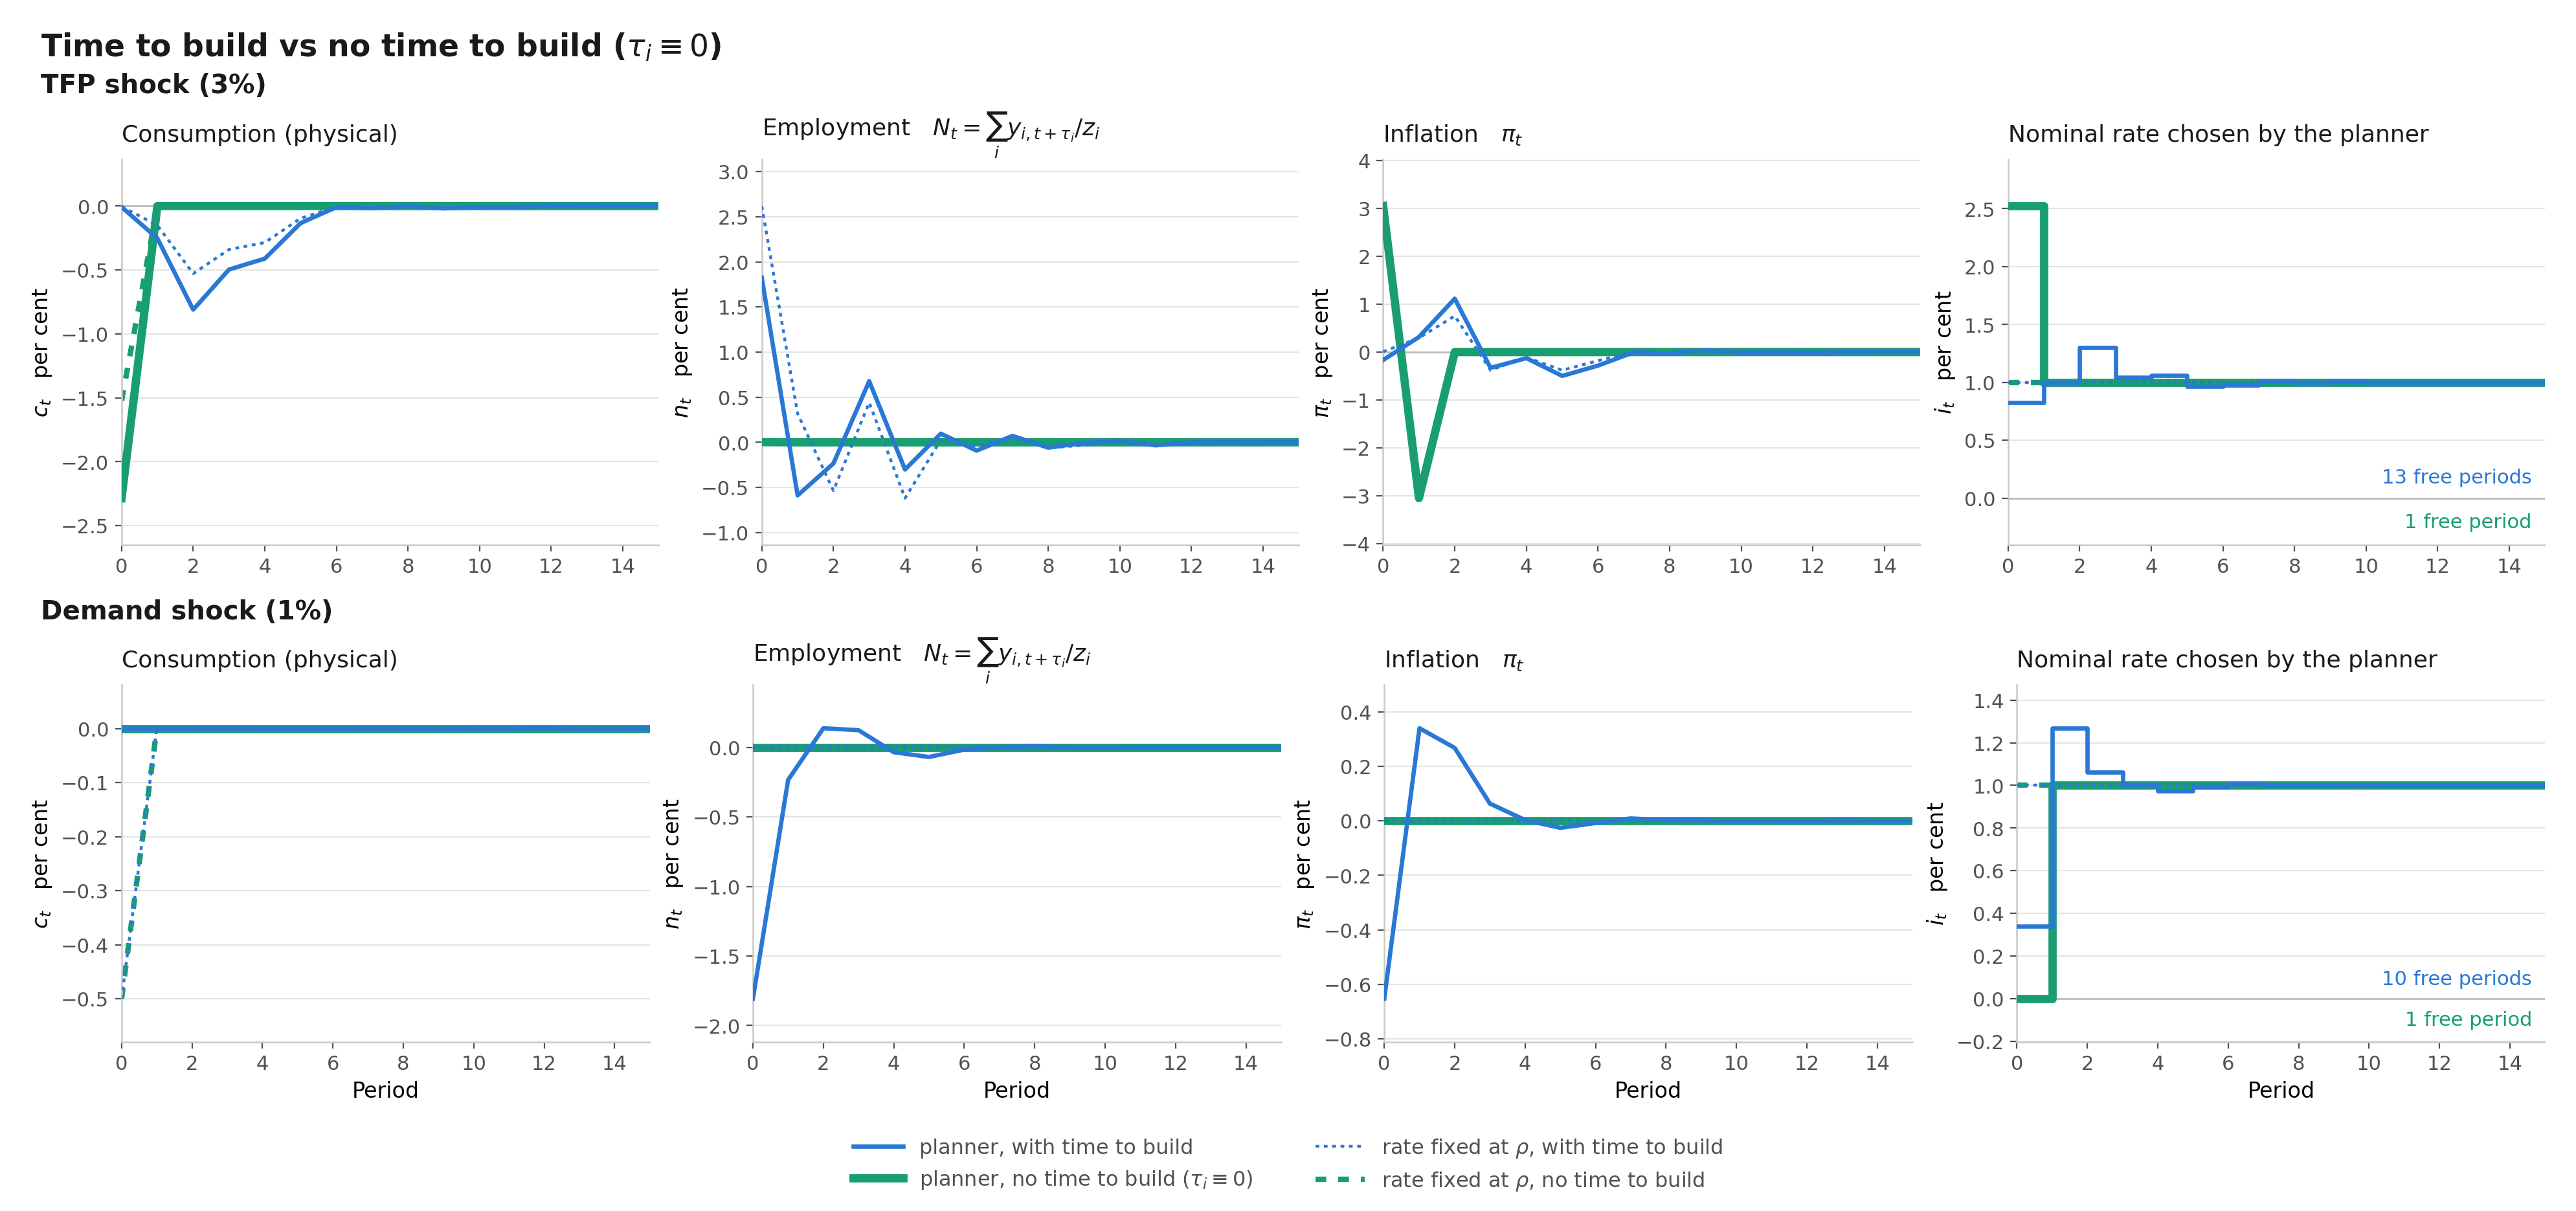
\includegraphics[width=\textwidth]{semi_endo_new_fixed_planner_ttb_vs_notb.png}
    \end{column}
    \begin{column}{0.25\textwidth}
      \textbf{\color{mgreen}$\tau_i\equiv0$}\\
      one move, $i_t=r^n_t$

      \bigskip
      \textbf{\color{mblue}Time to build}\\
      10--13 periods, oscillating
    \end{column}
  \end{columns}
\end{frame}

% --------------------------------------------------------------------
\begin{frame}{Cuts only: rate capped at $\rho$}
  \begin{columns}[c,onlytextwidth]
    \begin{column}{0.7\textwidth}
      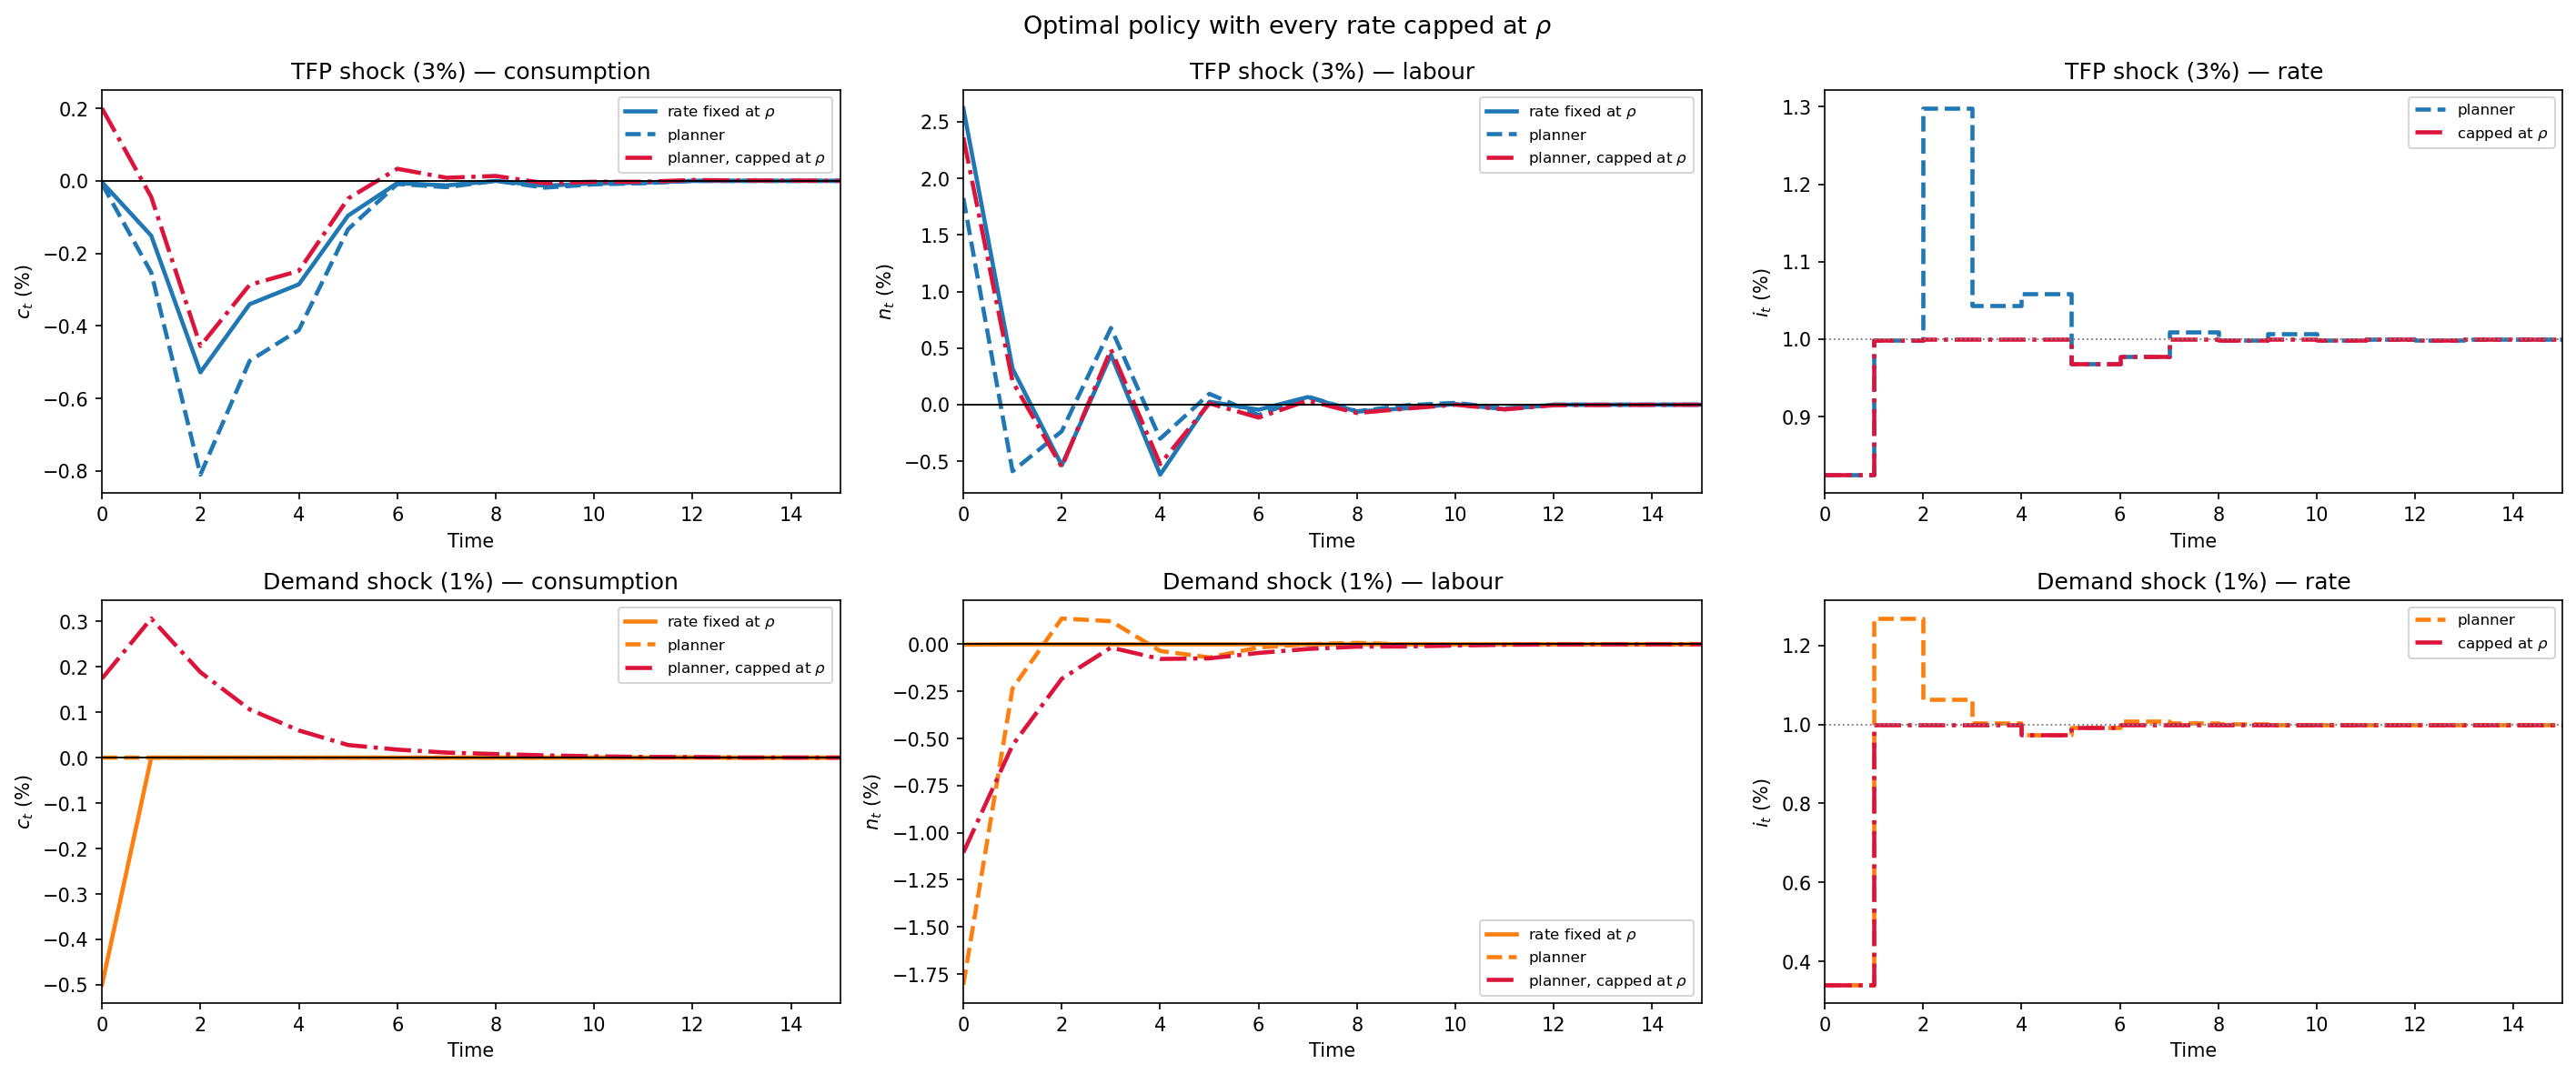
\includegraphics[width=\textwidth]{semi_endo_new_fixed_planner_capped.png}
    \end{column}
    \begin{column}{0.27\textwidth}
      \begin{itemize}\setlength{\itemsep}{0.7em}
        \item Consumption overshoots
        \item TFP: \ho{worse than the peg}
      \end{itemize}
    \end{column}
  \end{columns}
\end{frame}

% --------------------------------------------------------------------
\begin{frame}{$\gamma$ sets the sign of the TFP gap}
  \begin{columns}[c,onlytextwidth]
    \begin{column}{0.48\textwidth}
      Peg is loose iff
      \[
        \gamma\varphi_{ya}=\frac{\gamma(1+\eta)}{\gamma+\eta}>1\iff\gamma>1
      \]
      $\gamma=1$: peg is optimal.
    \end{column}
    \begin{column}{0.48\textwidth}
      \centering
      \begin{tabular}{rrr}
        \toprule
        $\gamma$ & $\gamma\varphi_{ya}$ & gap, \%\\
        \midrule
        0.50 & 0.60 & $-0.82$\\
        0.75 & 0.82 & $-0.23$\\
        1.00 & 1.00 & $+0.03$\\
        1.50 & 1.29 & $+0.22$\\
        \hl{2.00} & \hl{1.50} & \hl{$+0.28$}\\
        3.00 & 1.80 & $+0.30$\\
        \bottomrule
      \end{tabular}
    \end{column}
  \end{columns}
\end{frame}

% ==================================================================== PART II
\begin{frame}[plain]
  \vfill
  {\usebeamerfont{title}\color{ink}Unexpected shocks\par}
  \smallskip
  {\Large\color{mblue}Quantities committed in advance\par}
  \vfill
\end{frame}

% --------------------------------------------------------------------
\begin{frame}{Who can respond}
  \begin{columns}[c,onlytextwidth]
    \begin{column}{0.5\textwidth}
      $y_{i,t}$ chosen at $t-\tau_i$:
      \begin{itemize}\setlength{\itemsep}{0.5em}
        \item $\tau_i>t$: \hl{locked} at $y_i^{ss}$,\;
              $p_{i,t}=P_t\bigl(y_i^{ss}/Y_t\bigr)^{-1/\sigma}$
        \item $\tau_i\le t$: \hl{free}, prices at cost
      \end{itemize}
      \medskip
      Labour is free from $t=0$.
    \end{column}
    \begin{column}{0.46\textwidth}
      \centering
      \begin{tabular}{rrr}
        \toprule
        $t$ & free & locked share of $Y$\\
        \midrule
        0 & 1   & 99.1\%\\
        1 & 32  & 77.2\%\\
        2 & 129 & 32.5\%\\
        13 & 269 & 0\%\\
        \bottomrule
      \end{tabular}
    \end{column}
  \end{columns}
\end{frame}

% --------------------------------------------------------------------
\begin{frame}{Unexpected demand shock (1\%), peg}
  \fullfig{demand_unexpected_agg.png}
  \begin{itemize}
    \item Impact: \hl{$P_0=-0.93\%$, $Y_0=-0.03\%$}
  \end{itemize}
\end{frame}

% --------------------------------------------------------------------
\begin{frame}{Unexpected demand shock: by production lag}
  \fullfig{demand_unexpected_firms.png}
  \begin{itemize}
    \item Deliveries move at $t=\tau_i$; labour moves at $t=0$
  \end{itemize}
\end{frame}

% --------------------------------------------------------------------
\begin{frame}{Unexpected TFP shock (3\%, one period)}
  \fullfig{ss_A_cohorts.png}
  \begin{itemize}
    \item Trough \hl{$-0.66\%$ at $t=2$}; no time to build: \ho{$-2.28\%$ at $t=0$}
  \end{itemize}
\end{frame}

% --------------------------------------------------------------------
\begin{frame}{Unexpected TFP shock: by production lag}
  \fullfig{tfp_unexpected_firms.png}
  \begin{itemize}
    \item Damaged batch arrives at $t=\tau_i$
  \end{itemize}
\end{frame}

% --------------------------------------------------------------------
\begin{frame}{Reading the by-lag figures}
  One line per production lag $\tau=0,\dots,5$ (mean over firms with that $\tau$).
  \[
    \text{left:}\quad 100\,\log\frac{y_{\tau,t}}{y_{\tau}^{ss}}
    \qquad\qquad
    \text{right:}\quad 100\,\log\frac{l_{\tau,t}}{l_{\tau}^{ss}}
  \]
  \begin{itemize}\setlength{\itemsep}{0.7em}
    \item Left: \hl{output delivered at $t$}, relative to steady state
    \item Right: \ho{labour hired at $t$}, relative to steady state
    \item Line $\tau$: delivered output cannot move before $t=\tau$; labour moves from $t=0$
  \end{itemize}
\end{frame}

% --------------------------------------------------------------------
\begin{frame}{Fixed vs flexible wage, peg}
  \begin{center}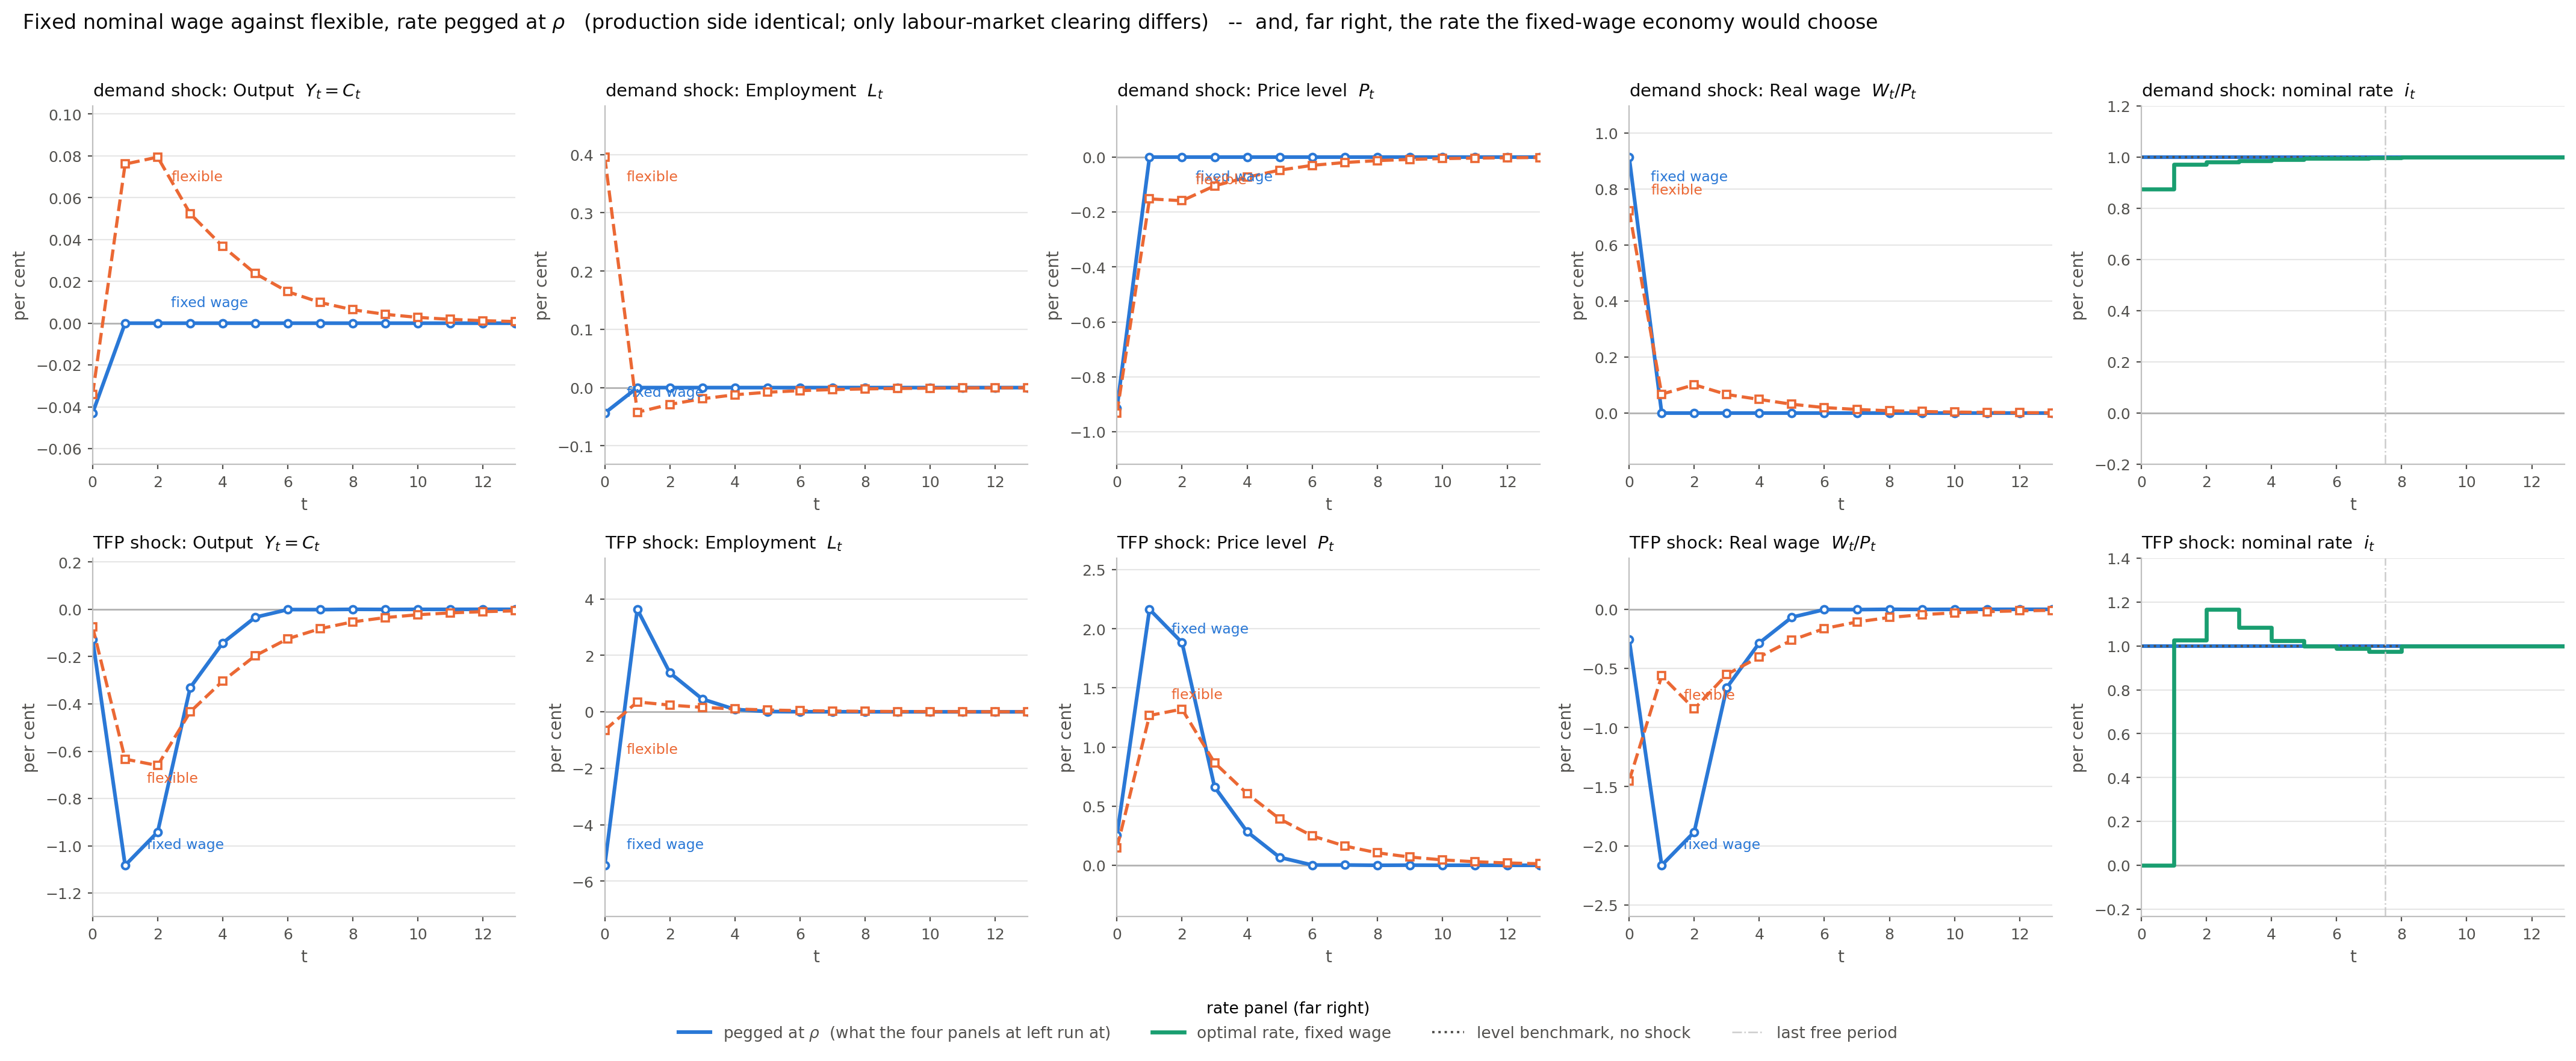
\includegraphics[width=\textwidth,height=0.66\textheight,keepaspectratio]{ss_fixed_wage_cohorts.png}\end{center}
  \vspace{-0.8em}
  \begin{itemize}
    \item TFP: peak employment $5.4\%$ vs $0.65\%$
  \end{itemize}
\end{frame}

% --------------------------------------------------------------------
\begin{frame}{Optimal rate, fixed wage}
  \centering
  \begin{tabular}{lrrrrrr}
    \toprule
    & \multicolumn{2}{c}{peak $|Y|$, \%} & \multicolumn{2}{c}{peak wedge, \%} & $i^*_0$ & gain, \% of $C$\\
    \cmidrule(lr){2-3}\cmidrule(lr){4-5}
    & peg & opt. & peg & opt. & & \\
    \midrule
    demand & 0.043 & 0.079 & 1.09 & 0.02 & 0.875\% & $0.00009$\\
    TFP    & 1.083 & 0.828 & 10.88 & 5.14 & 0\% & $0.0107$\\
    \bottomrule
  \end{tabular}

  \bigskip
  \raggedright
  \begin{itemize}
    \item Demand: small cut closes the wedge
    \item TFP: \hl{zero bound at $t=0$}, then above $\rho$
  \end{itemize}
\end{frame}

% --------------------------------------------------------------------
\begin{frame}{Optimal rate, fixed wage: demand shock}
  \fullfig{fixed_wage_optimal_demand.png}
  \begin{itemize}
    \item Cut to \hl{$0.875\%$ at $t=0$}; wedge $1.09\%\to0.02\%$
  \end{itemize}
\end{frame}

% --------------------------------------------------------------------
\begin{frame}{Optimal rate, fixed wage: TFP shock}
  \fullfig{fixed_wage_optimal_tfp.png}
  \begin{itemize}
    \item \hl{Zero at $t=0$}, then above $\rho$; peak employment $5.4\%\to2.9\%$
  \end{itemize}
\end{frame}

% --------------------------------------------------------------------
\begin{frame}{Optimal rate, fixed wage: with a markup}
  \begin{center}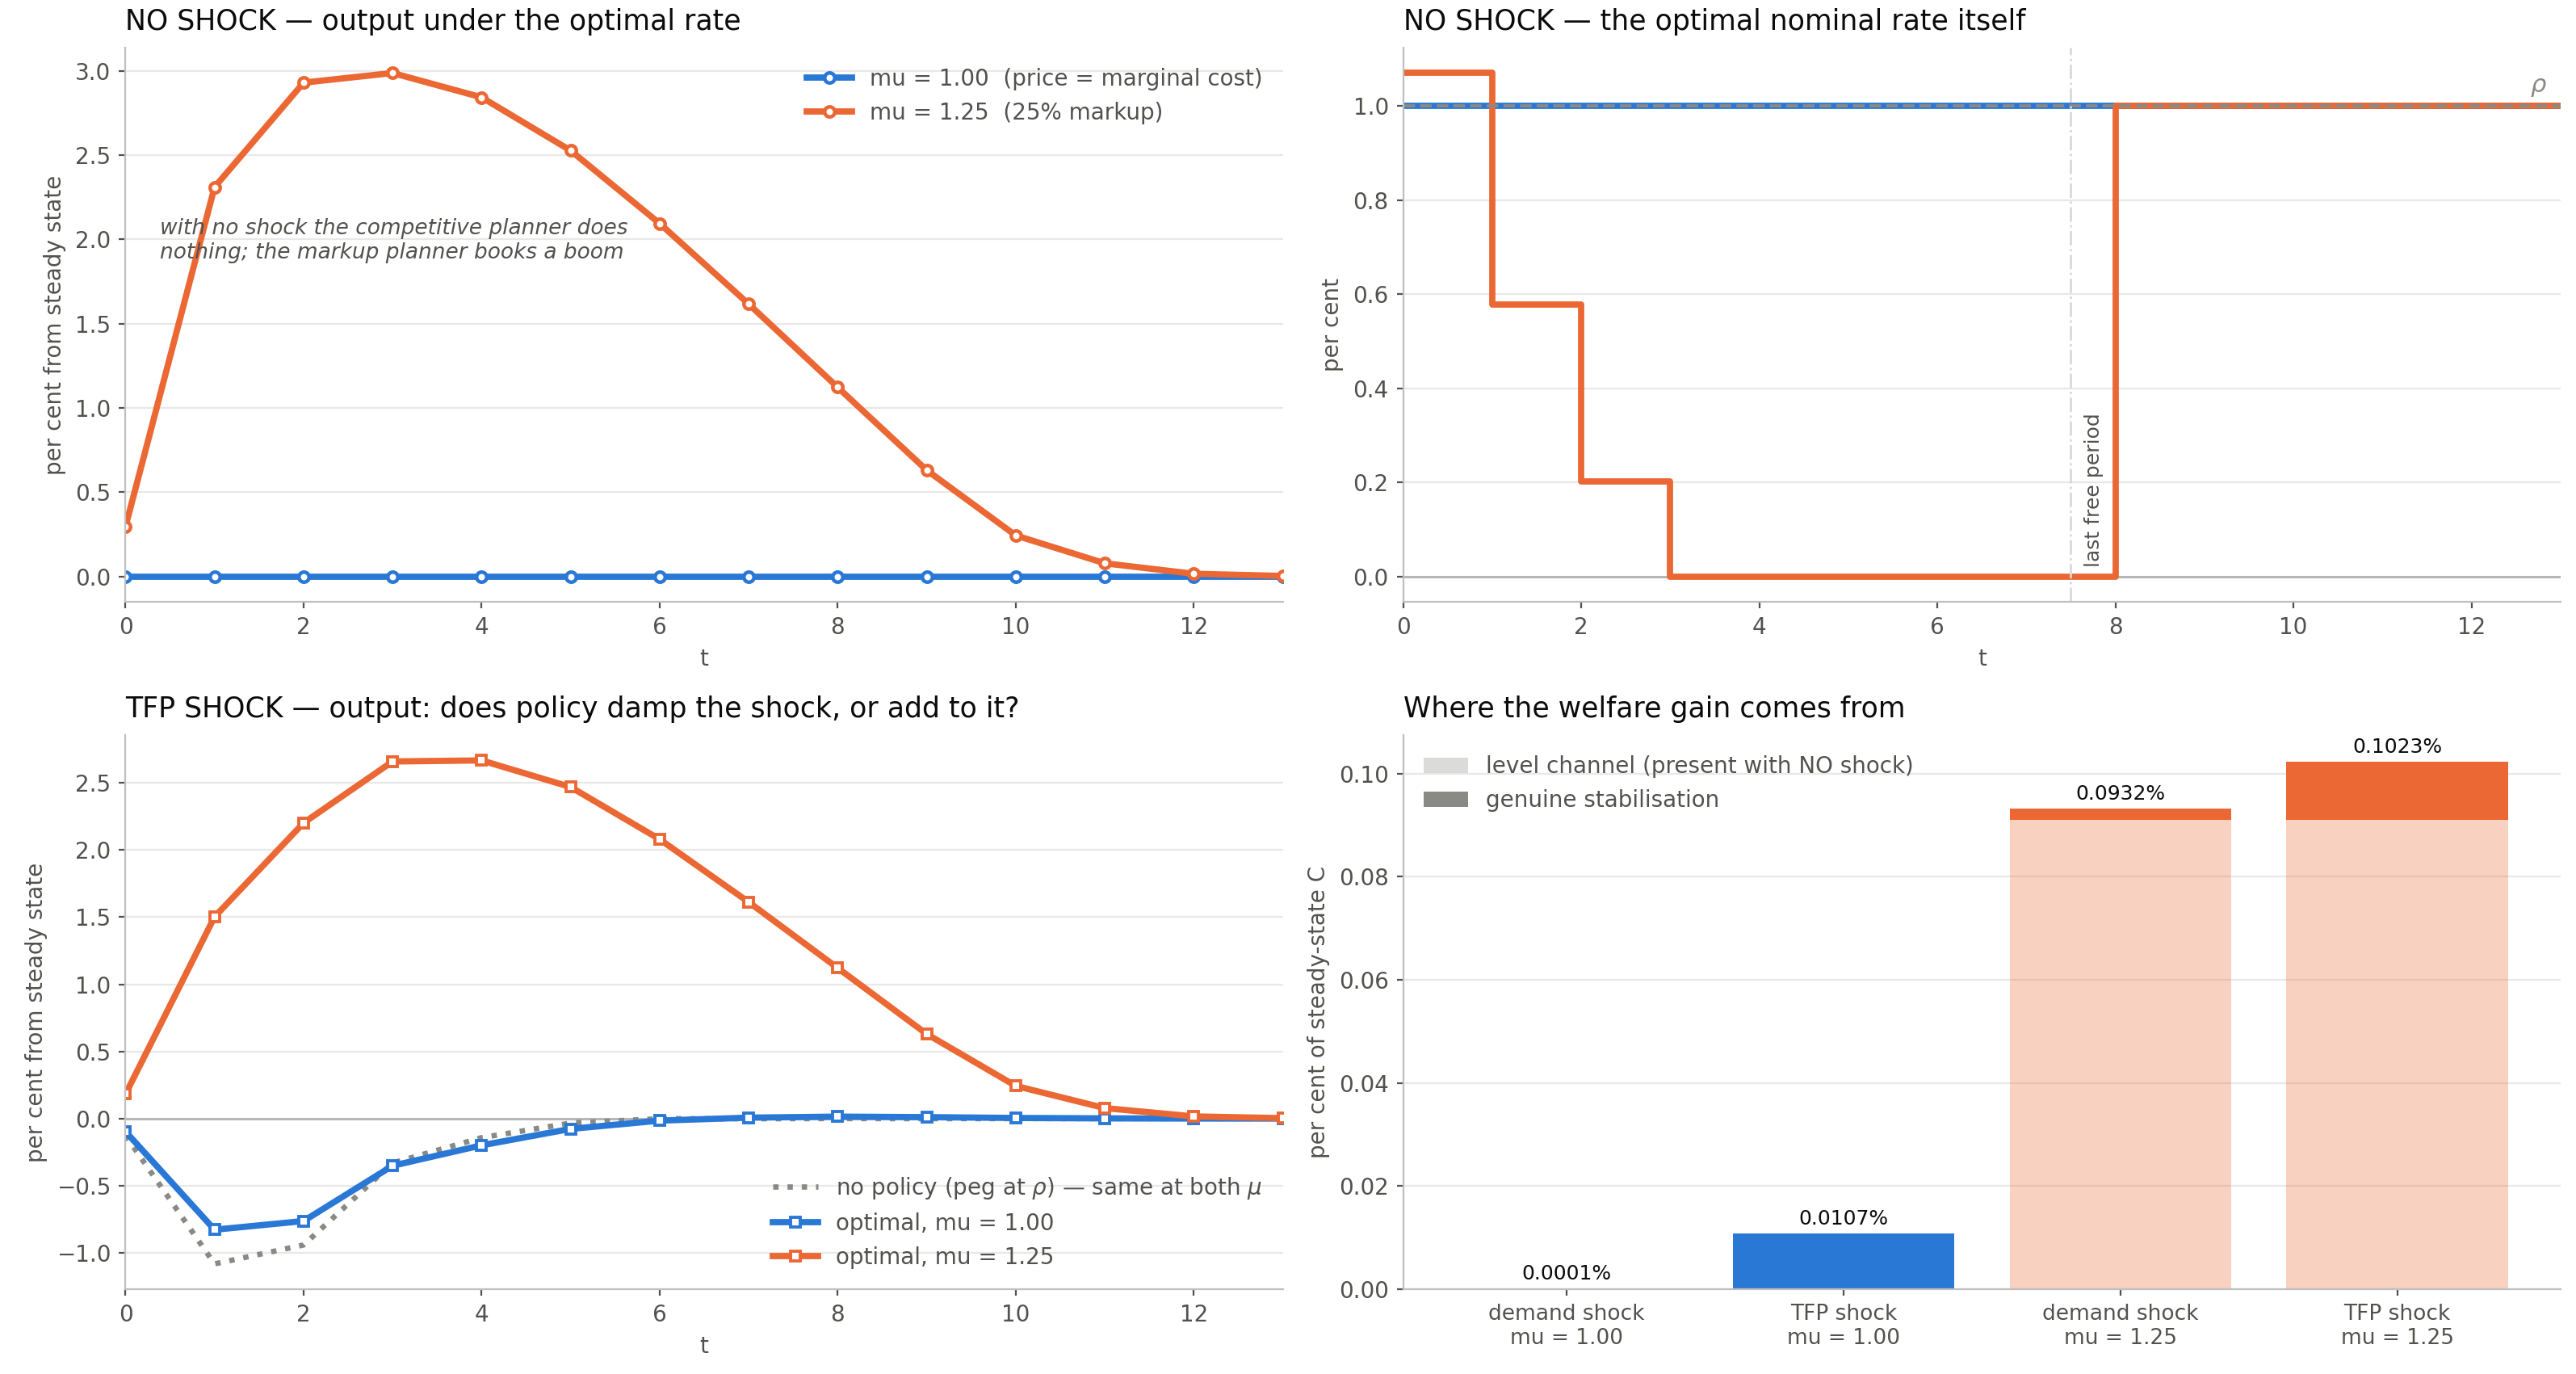
\includegraphics[width=\textwidth,height=0.68\textheight,keepaspectratio]{fixed_wage_optimal_markup.png}\end{center}
  \vspace{-0.8em}
  \begin{itemize}
    \item $\mu=1.25$, no shock: rate to zero, \ho{output $+3\%$}; $\mu=1$: stays at $\rho$
    \item Gain $0.09$--$0.10\%$ of $C$, about $90\%$ of it without any shock
  \end{itemize}
\end{frame}

% --------------------------------------------------------------------
\begin{frame}{Markup: the boom comes from $\chi$}
  \[
    \chi N^{\eta}C^{\gamma}=\frac{W}{P}=\frac{A}{\mu}
    \qquad\Longrightarrow\qquad
    C=N=A=1\ \text{ needs }\ \hl{$\chi=1/\mu$}
  \]
  \centering
  \begin{tabular}{lcc}
    \toprule
    no shock, $\mu=1.25$, 8 free periods & $\chi=1$ & $\chi=1/\mu$\\
    \midrule
    expected shocks   & $i^*=\rho$ & \ho{$i^*=0$, $C$ $+4.5\%$}\\
    unexpected shocks & $i^*=\rho$ & \ho{$i^*\to0$, $Y$ $+3.0\%$}\\
    \bottomrule
  \end{tabular}

  \bigskip
  \raggedright
  \begin{itemize}
    \item $\chi=1/\mu$: employment below efficient, planner cuts
    \item $\chi=1$: efficient steady state (subsidy offsets the markup); $\mu$ drops out
    \item Normalising the steady state alone changes nothing
  \end{itemize}
\end{frame}

% --------------------------------------------------------------------
\begin{frame}{$\chi=1/\mu$: the boom lasts as long as the window}
  No shock, unexpected-shock model, 8 $\to$ 16 free periods.

  \medskip
  \centering
  \begin{tabular}{lccc}
    \toprule
    $\mu$ & $i^*_0$, \% & periods at zero & peak $Y$, \%\\
    \midrule
    1.00 & $1.00\to1.00$ & $0\to0$ & $0\to0$\\
    1.05 & $1.07\to1.17$ & $0\to0$ & $0.82\to1.13$\\
    1.15 & $1.18\to1.48$ & $2\to3$ & $2.26\to3.21$\\
    1.25 & $1.07\to1.72$ & $5\to7$ & $2.99\to4.86$\\
    1.50 & $0.41\to1.65$ & $7\to13$ & $3.51\to6.76$\\
    \bottomrule
  \end{tabular}

  \bigskip
  \raggedright
  \begin{itemize}
    \item Wage fixed forever, inflation free: nothing ends the boom but the peg
  \end{itemize}
\end{frame}

% --------------------------------------------------------------------
\begin{frame}{$\chi=1/\mu$: the response to the shock}
  $i^*_0(\text{shock})-i^*_0(\text{no shock})$, pp, 8 $\to$ 16 free periods.

  \medskip
  \centering
  \begin{tabular}{lcc}
    \toprule
    $\mu$ & demand & TFP\\
    \midrule
    1.00 & $-0.125\to-0.125$ & $-1.00\to-1.00$\\
    1.15 & $-0.128\to-0.129$ & $-1.18\to-1.48$\\
    1.25 & $-0.132\to-0.131$ & $-1.07\to-1.72$\\
    1.50 & $-0.144\to-0.137$ & $-0.41\to-1.65$\\
    \bottomrule
  \end{tabular}

  \bigskip
  \raggedright
  \begin{itemize}
    \item Demand: same cut at every $\mu$ and window
    \item TFP: $i^*_0=0$ at every $\mu$
    \item Gain at $\mu=1.25$, \% of $C$: boom $0.091$; shock $0.002$ (demand), $0.011$ (TFP)
  \end{itemize}
\end{frame}

% --------------------------------------------------------------------
\begin{frame}{Inflation bias}
  \begin{itemize}\setlength{\itemsep}{0.9em}
    \item $\chi=1/\mu$: steady state inefficient, planner cuts whenever it is free
    \item Return to $\rho$ is imposed: longer window, longer boom
    \item \hl{Classical inflation-bias problem}
    \item Next: solve the commitment problem in this setting
  \end{itemize}
\end{frame}

% ==================================================================== END
% --------------------------------------------------------------------
\begin{frame}{Summary}
  \begin{itemize}\setlength{\itemsep}{0.9em}
    \item \hl{Expected}: rate moves echo for 13 periods; optimal path cuts, then overshoots
    \item Planner reaches $|c-c^e|\sim10^{-6}$; gain $\sim10^{-4}\%$ of $C$
    \item \hl{Unexpected} demand: prices $-0.93\%$, output $-0.03\%$
    \item \hl{Unexpected} TFP: trough at $t=2$, not on impact
    \item Rate neutral with flexible wage, not with fixed wage
  \end{itemize}
\end{frame}

\end{document}
